\chapter{Aqueous chemistry of the rare earth elements (REE)}\label{chap:REE_aq_chem}
\chaptermark{REE aqueous chemistry}

\section{What are the REE?}

The REE constitute much of Group 3 of the periodic table, a group of 16 transition metals, including the lanthanide series (La to Lu, excluding Pm), Yttrium (Y) and Scandium (Sc).
The ``rare'' moniker stems from their initial isolation from uncommon mineral phases in the 18th and 19th century \citep{CastorHedrick}, though the natural abundance of REE in the earth's crust range from 0.52 parts per million (ppm) to 41.5 ppm, in the same range as Pb or Sn and exceeding the natural, crustal abundance of Ag and Hg \citep{CRC}.

In the natural sciences, predictable thermodynamic differences between the REE make these elements uniquely capable tools for interpreting natural geologic and chemical processes \citep{Murray_Geol_1990, Laveuf_Geoderma_2009}.
Rare earth lithogeochemistries have long been used to infer depositional environments of geologic strata \citep{Murray_Geol_1990, PAAS, Hanson_AREPS_1980}.
Similarly, REE serve as benign analogs to the transuranic actinide series for nuclear waste disposal studies \citep{Krauskopf_CG_1986, Millero_GCA_1992};
as potential markers of regional authenticity for high value exported food products such as wine, pumpkin-seed oil, and olive oil \citep{Jakubowski_FJAC_1999, Joebstl_FC_2010, Farmaki_AL_2012};
and for studying mixing and metal cycling in the oceans \citep{DeBaar_Nature_1983, Elderfield_PTRS_1988}.

Many of the same properties that yield the unique and predictable geochemistry of the REE have lead to their use in more consumer products than nearly any other element group \citep{CastorHedrick, Graedel_PNAS_2015a}. In most applications, the performance of the REE is unmatched \citep{Ciacci_EST_2015, Nassar_JIE_2015}, making substitution (with more readily available/environmentally benign elements) undesirable.

Based on atomic number, the REE are segregated into light and heavy REE (LREE and HREE, respectively) with the division occurring between Eu and Gd \citep{CastorHedrick};
some studies further distinguish middle REE (MREE), though the specific elements are inconsistently defined between authors \citep{Hannigan_CG_2001, Tang_CG_2010, Choi_CG_2009}.
These ``weight'' distinctions allow for simplified description and quantification of the inter-element relationships, typically ratios of normalized concentrations, which are exploited in REE analysis.
Similarly, anomalies of certain REE --- due to redox lability for Ce and Eu \citep{Brookins_RMG_1989} and large anthropogenic emissions for Gd \citep{Bau_EPSL_1996} --- are used to interpret geochemical processes.
Y and Sc exhibit similar properties to the lanthanides and are thus included in the suite of REE with Y being most similar to HREE and Sc being most similar to LREE in solution \citep{Brookins_RMG_1989}.

\section{REE speciation in natural waters}

The speciation of dissolved metals governs their reactivity in aqueous systems with respect to solid precipitation/dissolution, oxidation/reduction, microbial processes, and surface processes including ion exchange and surface complexation.
Thus it is crucial to understand the speciation of the REE in the proposed matrices to maximize extraction and interpret experimental results.
The REE exist almost exclusively in a 3+ oxidation state, though Ce is readily oxidized to a 4+ state under oxic conditions and Eu is reduced to a 2+ state under extreme reducing conditions or at high temperatures ($T \sim 200^\circ$C).

While not indicative in isolation of how the REE with speciate, trends in stability constants for various ligands can be compared to assess reactivity.
Thermodynamic data for the REE, compiled from the literature, are shown in Figure~\ref{fig:REE-stab-consts}.
From these data, the following order of reactivity is observed for the common, inorganic ligands (i.e. not DTPA): \ce{PO4^3- >> CO3^2- > OH- > F- / SO4^2- >> NO3- / Cl-}.
This order agrees with the general trend of hardness described by \citet{Pearson_JACS_1963}.
However, since \ce{PO4^3-} is significantly less abundant in natural waters than \ce{CO3^2-}, carbonate complexes are generally understood to be the predominant species of the dissolved REE \citep{Johannesson_LO_1994, Johannesson_AG_1995}.

\begin{figure}[htbp]
\begin{center}
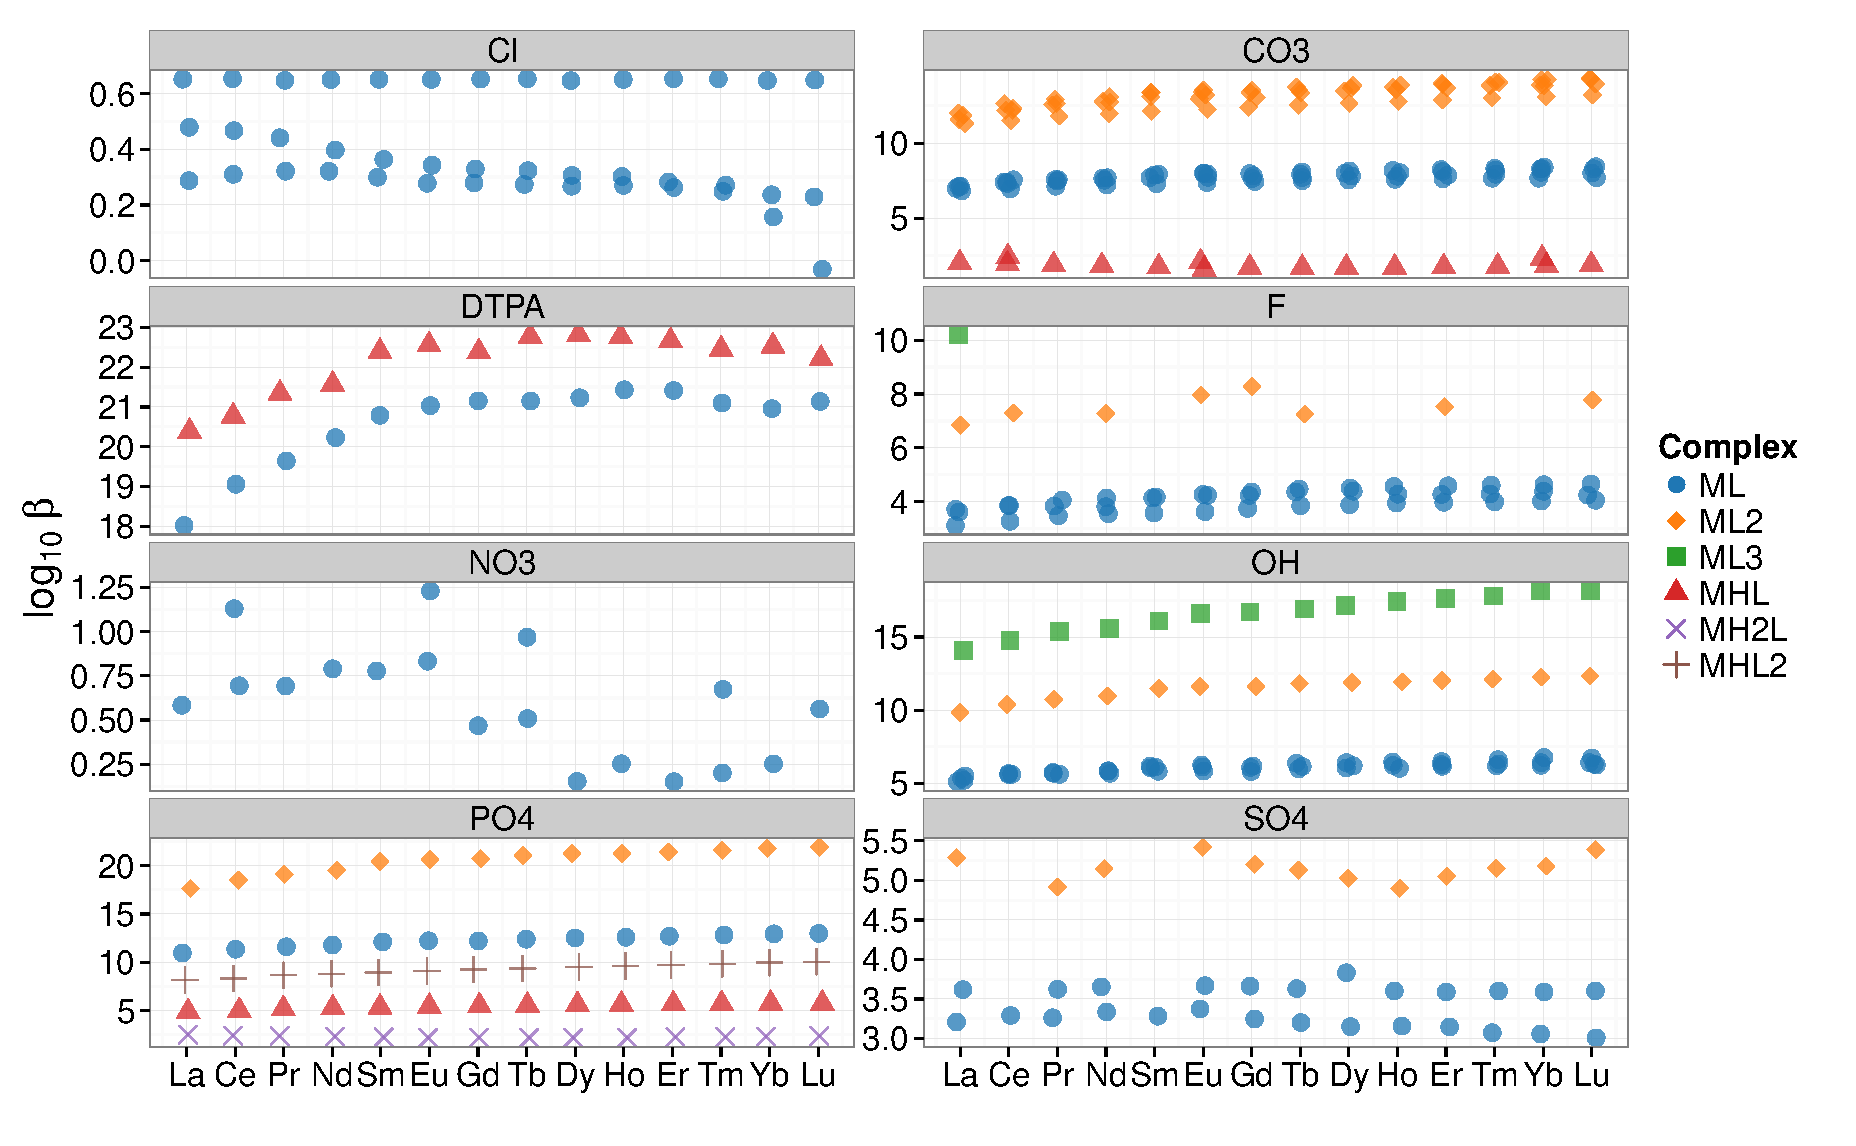
\includegraphics[width = \textwidth]{REE-aq-chem-figs/REE-stab-const-freeY.pdf}
\caption[REE-ligand complex formation constants ($\log_{10} \beta$) compiled from published literature.]{REE-ligand complex formation constants ($\log_{10} \beta$) compiled from published literature \citep{Wood_CG_1990, Lee_GCA_1992, Millero_GCA_1992, Liu_JSC_1998, Klugness_Poly_2000, Luo_JSC_2000, Luo_JSC_2001, Grimes_JSC_2014}. Stability constant values are for the general reaction:
\ce{M^3+ + aH+ + bL^z- <=>[\beta] MH_aL_b^{(3+ a - bz)}}.
Data are not available for all complexes of all elements.}
\label{fig:REE-stab-consts}
\end{center}
\end{figure}

A more practical scenario might be that of the model freshwater presented by \citet{Morel_Hering}:
\begin{center}
\begin{tabular}{cc}
$TOTNa = 10^{-3.55}\text{ M}$ & $TOTCl = 10^{-3.7}\text{ M}$\\
$TOTCa = 10^{-3.43}\text{ M}$ & $TOTSO_4 = 10^{-4}\text{ M}$\\
$TOTMg = 10^{-3.8}\text{ M}$ & $TOTCO_3 = 10^{-3}\text{ M}$\\
$TOTK = 10^{-4.22}\text{ M}$ &  \\
\end{tabular}
\end{center}
Speciation of three select REE (Nd, Gd, and Ho) in this system at median concentrations of those elements in grounwater \citep{Noack_EST_2014} is shown in Figure~\ref{fig:REE-spec-fresh}.
Under these conditions the free \ce{Ln^3+} species predominates to near pH 6, where the \ce{LnCO3+} species becomes the primary species.
As the solution becomes more basic (pH $>8$) the \ce{Ln(CO3)2-} and subsequently (pH $>$ 10) the \ce{Ln(OH)4^-} complexes predominate.
A small ($<25\%$) fraction of the REE are found as sulfate complexes at low pH, but these species are rapidly displaced by the carbonate species starting at pH 6.
While the practical manifestation is small, increased stability of the HREE-carbonate complexes (Figure~\ref{fig:REE-stab-consts}) is apparent as the conversion from $(\ce{Ln^3+} + \ce{LnSO4+})$ to \ce{LnCO3+} occurs at lower pH values from Nd to Gd to Ho.

\begin{figure}[htbp]
\begin{center}
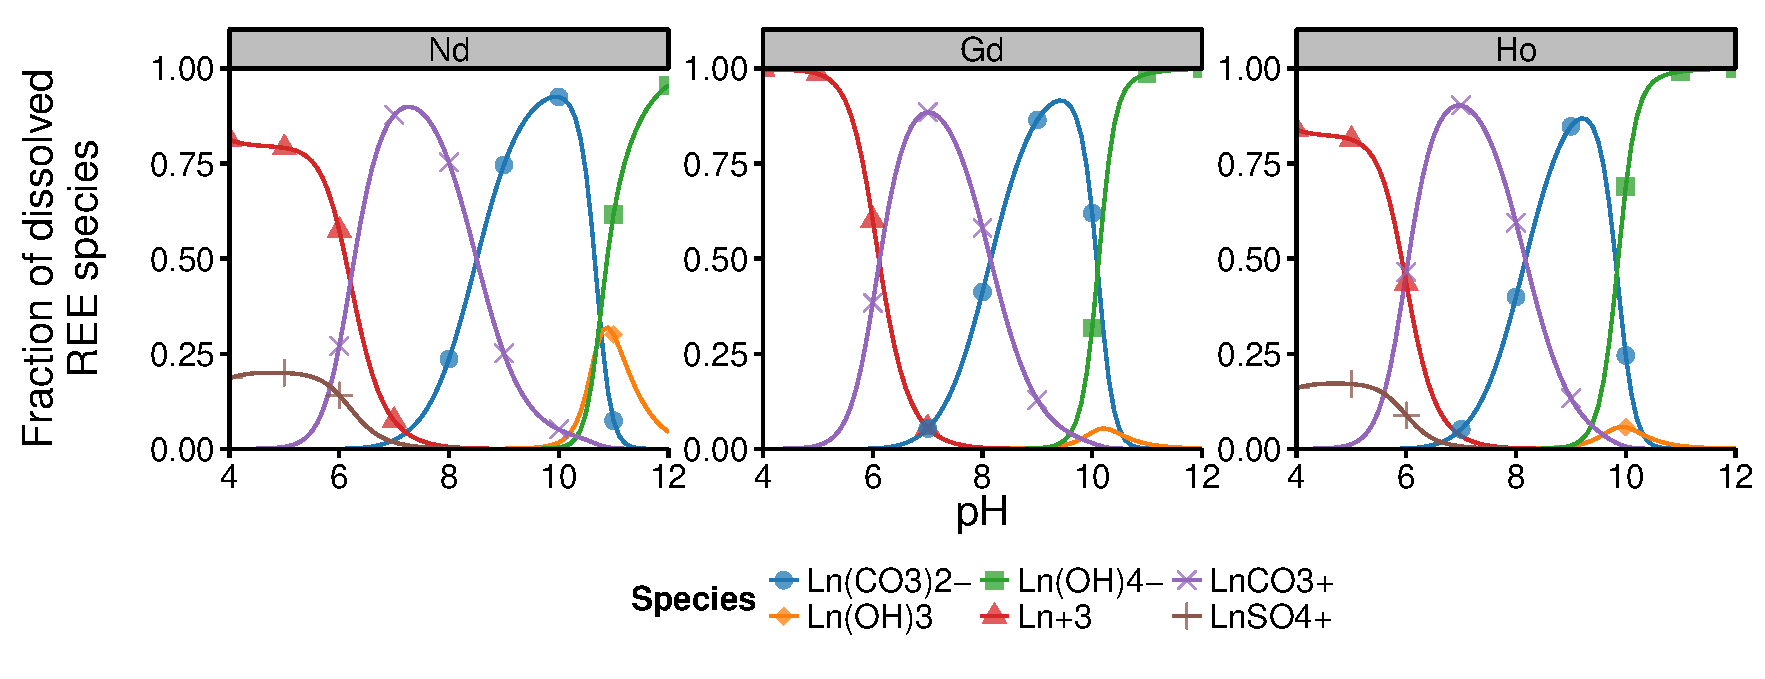
\includegraphics[width = \textwidth]{REE-aq-chem-figs/REE-spec-MH-freshwater-horiz.pdf}
\caption[Speciation of select REE in a model fresh water at 25$^\circ$C.]{Speciation of select REE in a model fresh water (Example 1, pg. 345 from \citet{Morel_Hering}) at 25$^\circ$C.
Speciation calculated using \texttt{PHREEQC} \citep{PHREEQC} in \texttt{R} \citep{R} with the \texttt{llnl.dat} thermodynamic database.
Total REE concentrations are the medians for the elements in groundwater \citep{Noack_EST_2014}: 263 ppt, 76 ppt, and 12 ppt for Nd, Gd, and Ho respectively.
Curves are labeled with plot markers at integer pH values for comparison.
Species that make up less than 5\% at their maximum are not plotted.}
\label{fig:REE-spec-fresh}
\end{center}
\end{figure}

This system can be compared to an average geothermal produced water \citep[average values from ][]{ProdWat}:
\begin{center}
\begin{tabular}{cc}
$TOTNa = 10^{-1.23}\text{ M}$ & $TOTCl = 10^{-1.14}\text{ M}$\\
$TOTCa = 10^{-2.65}\text{ M}$ & $TOTSO_4 = 10^{-2.45}\text{ M}$\\
$TOTMg = 10^{-2.53}\text{ M}$ & $TOTCO_3 = 10^{-2.37}\text{ M}$\\
$TOTK = 10^{-2.71}\text{ M}$ &  \\
\end{tabular}
\end{center}
The speciation of median REE concentrations in this system is shown as a function of pH in Figure~\ref{fig:REE-spec-geothermal}.
The primary difference between the speciation in this model geothermal water, compared to the freshwater system, is the increased prevalence of the \ce{LnSO4+} complexes at low pH (even overtaking the free ion for Nd).
However, even after the extraction of useable heat, geothermal waters remain quite hot ($T \sim 70-120^\circ$C).
This increase in temperature significantly alters the REE speciation for the same bulk solutes (Figure~\ref{fig:REE-spec-geothermal-hot} shows $T=90^\circ$C).
Here, the sulfate complexes persist to pH $\sim 7$, while the prevalence of the carbonate complexes is displaced by hydrolysis products.

\begin{figure}[htbp]
\begin{center}
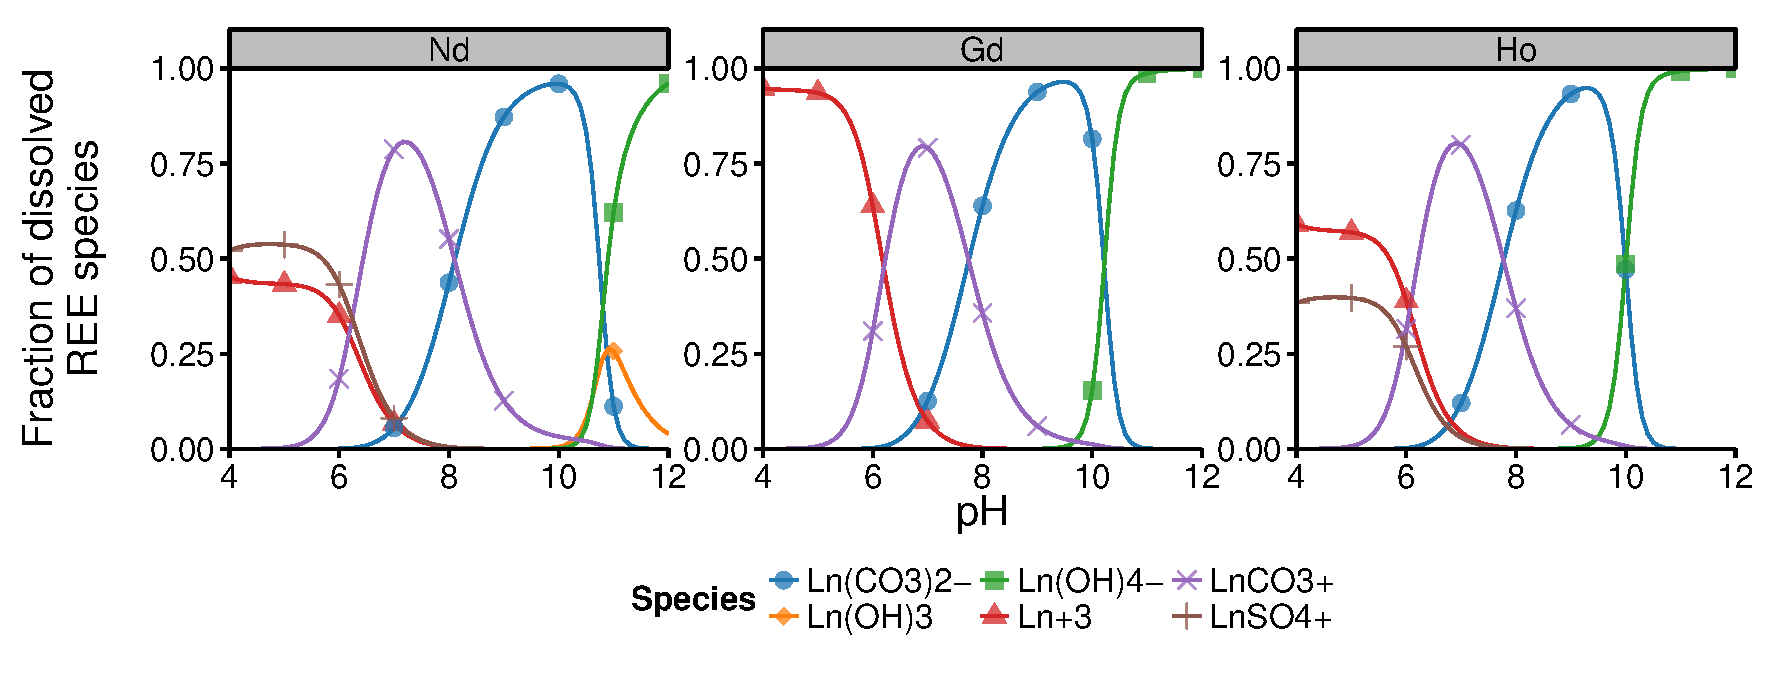
\includegraphics[width = \textwidth]{REE-aq-chem-figs/REE-spec-med-geothermal-horiz.pdf}
\caption[Speciation of select REE in a median geothermal water at 25$^\circ$C.]{Speciation of select REE in a median geothermal water (estimated from \citet{ProdWat}) at 25$^\circ$C.
Speciation calculated using \texttt{PHREEQC} \citep{PHREEQC} in \texttt{R} \citep{R} with the \texttt{llnl.dat} thermodynamic database.
Total REE concentrations are the medians for the elements in groundwater \citep{Noack_EST_2014}: 263 ppt, 76 ppt, and 12 ppt for Nd, Gd, and Ho respectively.
Curves are labeled with plot markers at integer pH values for comparison.
Species that make up less than 5\% at their maximum are not plotted.}
\label{fig:REE-spec-geothermal}
\end{center}
\end{figure}

\begin{figure}[htbp]
\begin{center}
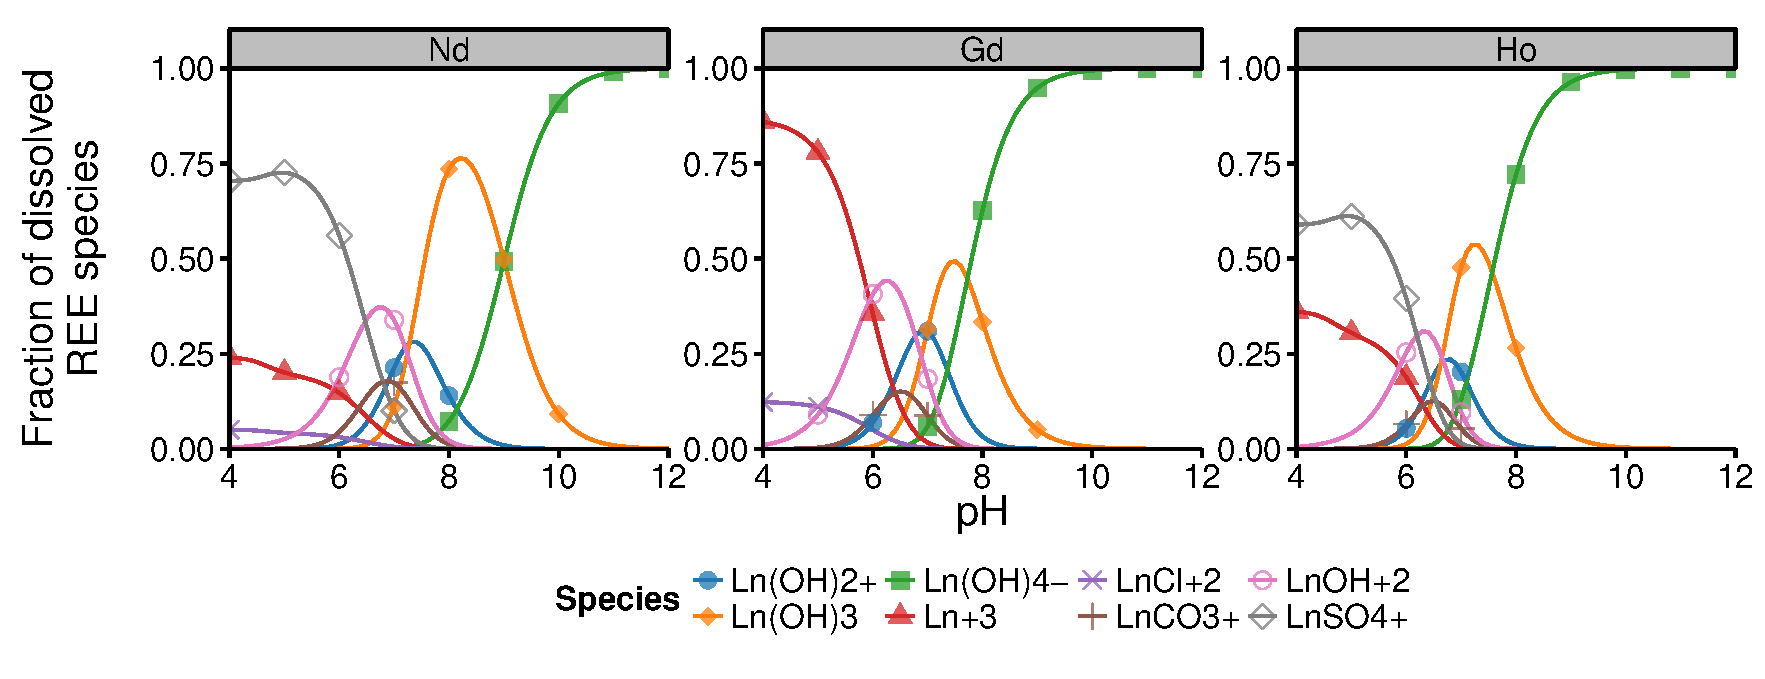
\includegraphics[width = \textwidth]{REE-aq-chem-figs/REE-spec-med-geothermal-90C-horiz.pdf}
\caption[Speciation of select REE in a median geothermal water at 90$^\circ$C.]{Speciation of select REE in a median geothermal water (estimated from \citet{ProdWat}) at 90$^\circ$C.
Speciation calculated using \texttt{PHREEQC} \citep{PHREEQC} in \texttt{R} \citep{R} with the \texttt{llnl.dat} thermodynamic database.
Total REE concentrations are the medians for the elements in groundwater \citep{Noack_EST_2014}: 263 ppt, 76 ppt, and 12 ppt for Nd, Gd, and Ho respectively.
Curves are labeled with plot markers at integer pH values for comparison.
Species that make up less than 5\% at their maximum are not plotted.}
\label{fig:REE-spec-geothermal-hot}
\end{center}
\end{figure}

If we instead consider the speciation of the REE in a simple salt solution matching the electrolyte composition of adsorption experiments detailed later in this thesis (0.5 m NaCl; \hyperref[CH5]{Chapter~\ref*{CH5}}), in the absence of carbonate, the free \ce{Ln^3+} species is predominant until pH $>8$ (Figure~\ref{fig:REE-spec-exp}).
Thus there should be little competition (for the functionalized adsorbents) in this system.
By treating the surface bound DTPA (1 mmol DTPA / g adsorbent, 10 g adsorbent / L solution) as an aqueous ligand (and using the stability constants from Figure~\ref{fig:REE-stab-consts}), the fraction of surface-bound REE can be estimated.
Figure~\ref{fig:REE-spec-exp} illustrates the high affinity of DTPA for the REE;
complete complexation as DTPA complexes is accomplished for all REE by pH 2.5.
Notably, at this pH the DTPA exists in a mixture of protonation states as \ce{H5DTPA}, \ce{H4DTPA-}, and \ce{H3DTPA^2-}.
While the fully deprotonated \ce{DTPA^5-} constitutes an insignificant portion of the total DTPA at pH 2.5 ($\log_{10}\alpha_{DTPA}= -15.2$),  the magnitude of the stability constant ($18 < \log_{10} \beta_{ML} < 21.4$) compensates for the mass action disadvantage.

\begin{figure}[htbp]
\begin{center}
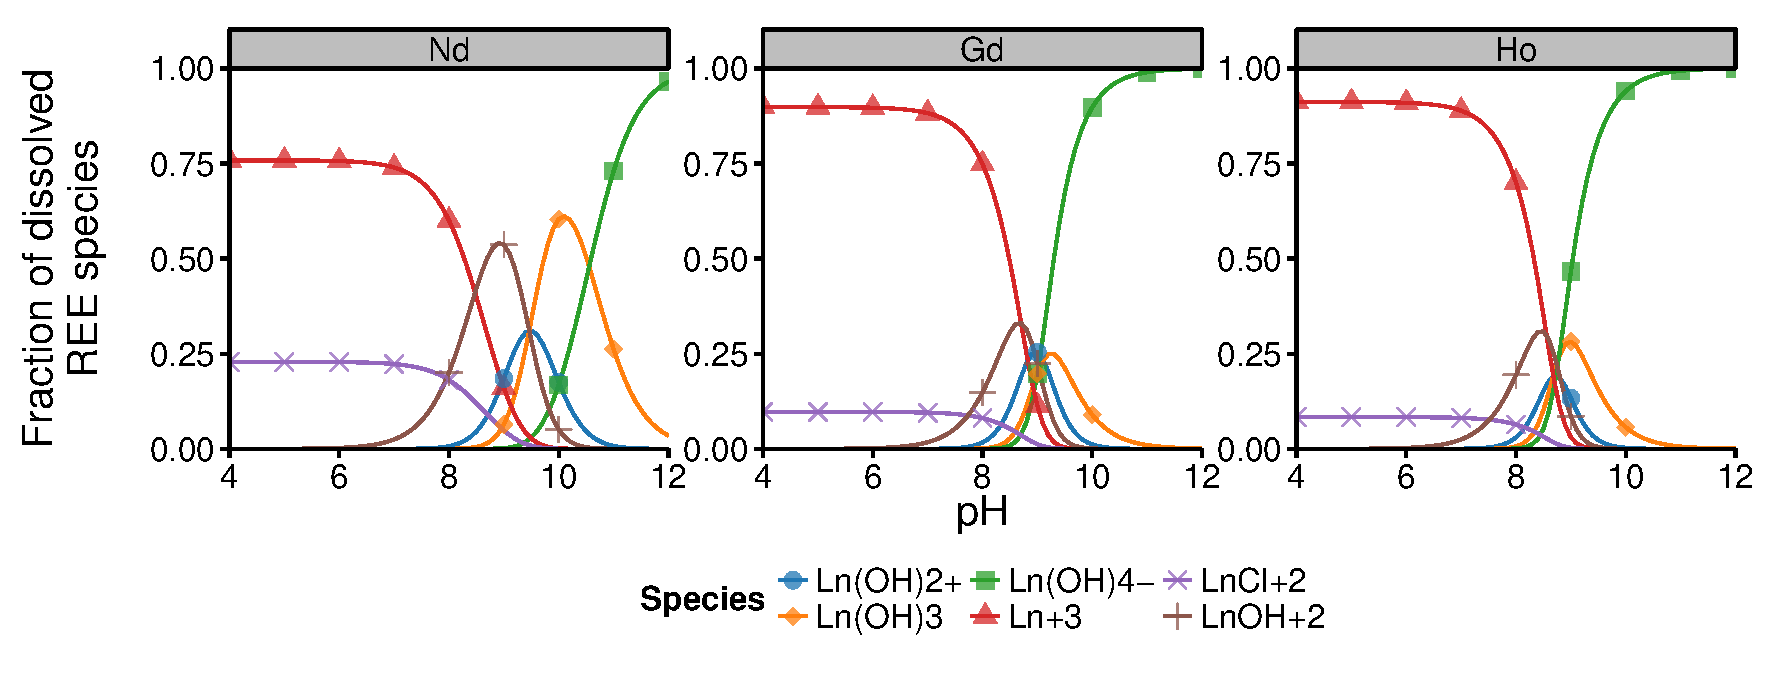
\includegraphics[width = \textwidth]{REE-aq-chem-figs/REE-spec-05mNaCl-horiz.pdf}
\caption[Speciation of select REE in 0.5 m NaCl at 25$^\circ$C.]{Speciation of select REE in 0.5 m NaCl (matching experimental electrolytes for adsorption tests in \hyperref[CH5]{Chapter~\ref*{CH5}}) at 25$^\circ$C.
Speciation calculated using \texttt{PHREEQC} \citep{PHREEQC} in \texttt{R} \citep{R} with the \texttt{llnl.dat} thermodynamic database.
Total REE concentrations are 100 ppb of each REE.
Curves are labeled with plot markers at integer pH values for comparison.
Species that make up less than 5\% at their maximum are not plotted.}
\label{fig:REE-spec-exp}
\end{center}
\end{figure}

\begin{figure}[htbp]\
\begin{center}
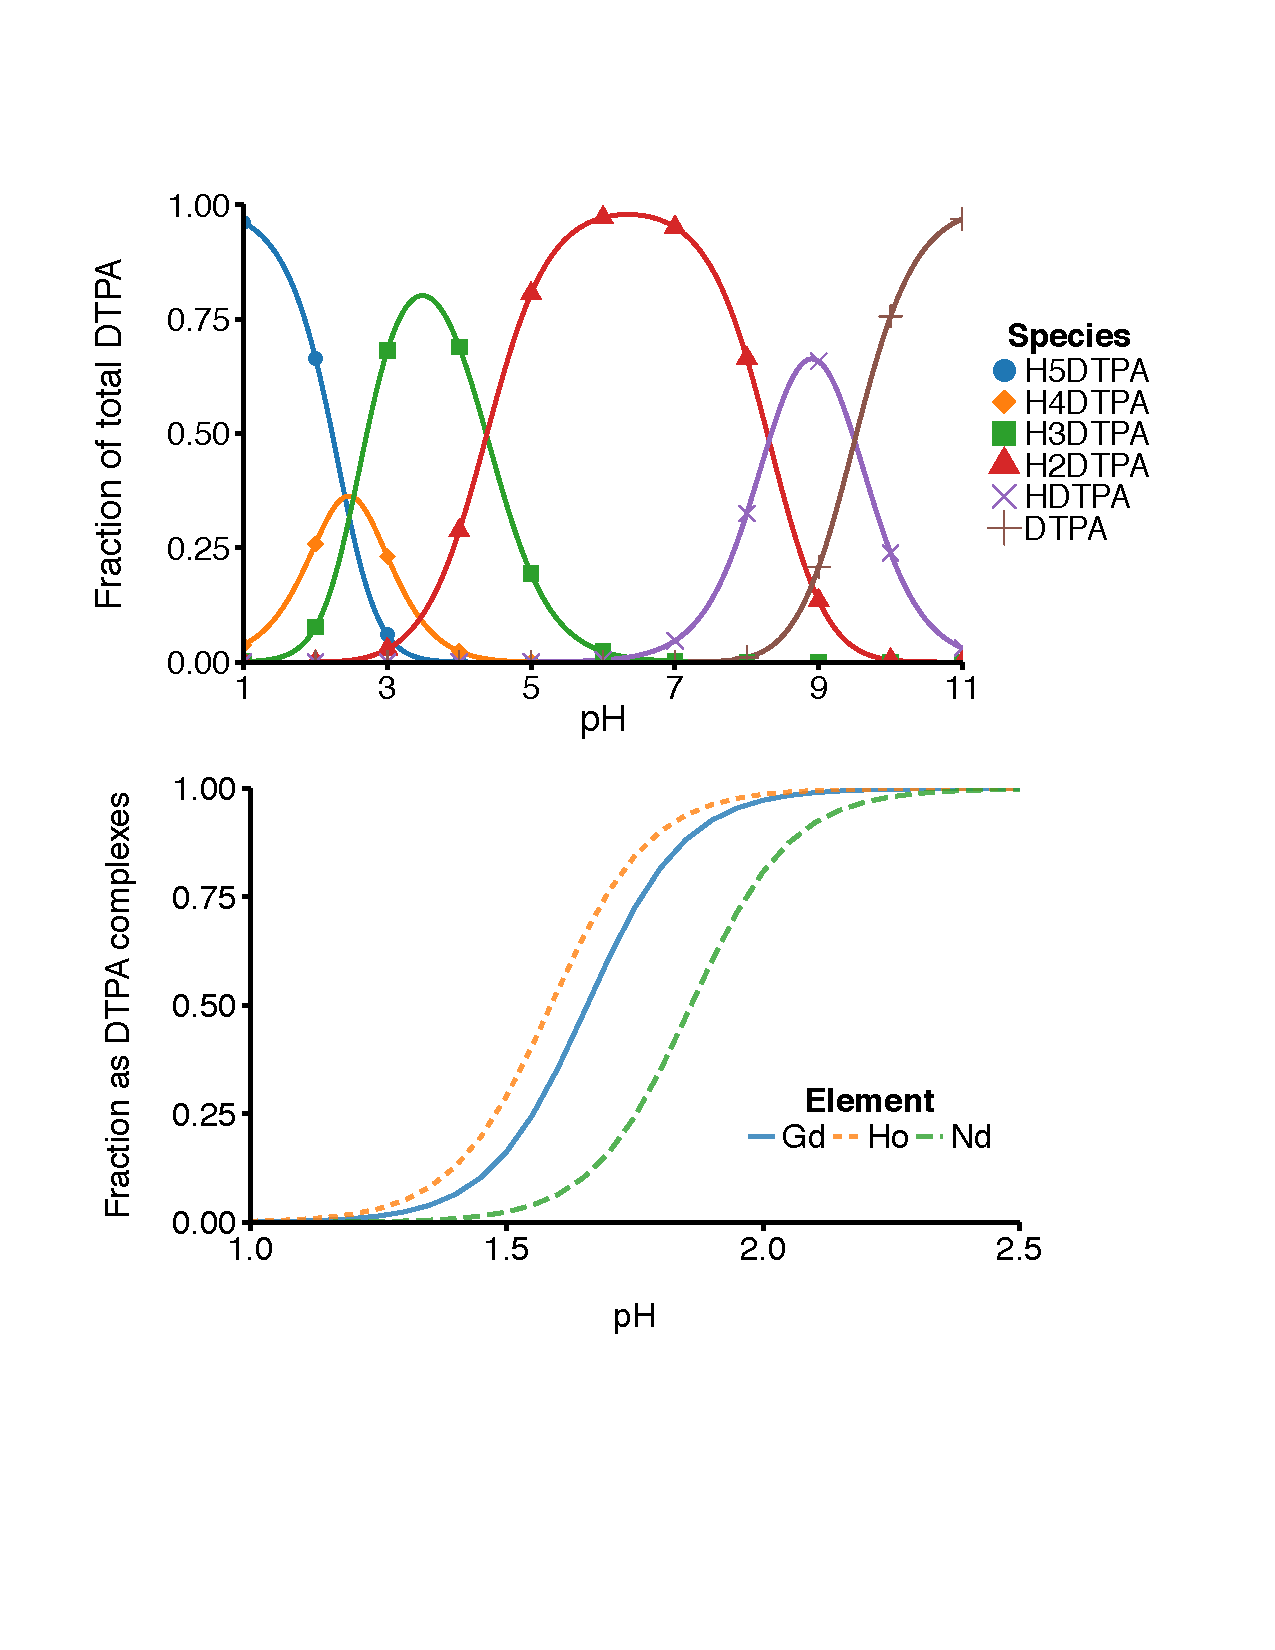
\includegraphics[width = 0.9\textwidth]{REE-aq-chem-figs/DTPA-model-figs-comb.pdf}		
\caption[Speciation of DTPA and the fraction of DTPA-associated, dissolved REE as a function of pH.]{Speciation of 10 mM DTPA (top) and the fraction of dissolved REE in DTPA complexes (sum of ML and MHL; bottom) as a function of pH.
Conditions of calculation are 0.5 m NaCl, 100 ppb total of each REE, and 10 mM total DTPA at 25$^\circ$C}
\label{fig:REE-spec-exp}
\end{center}
\end{figure}


\bibliographystyle{unsrtnat}
\bibliography{Ch2_bib}